\subsubsection{Client}
\setclass{BubbleAndEat::Customer::Client}
\paragraph[::Client]{\class}\mbox{}\\ \label{\class}
\begin{figure}[H]
	\centering
	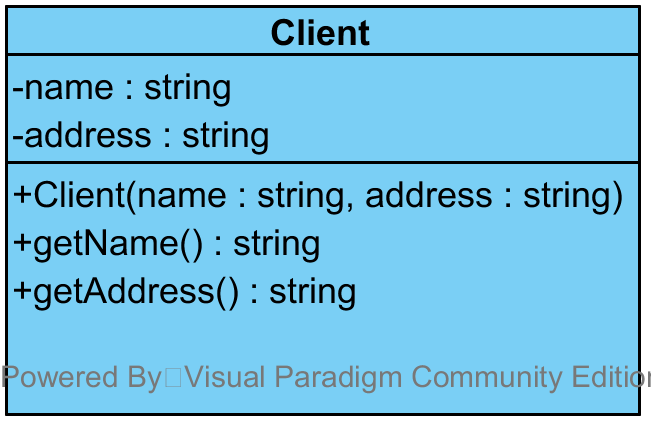
\includegraphics[width=7cm]{./diagrammi/demo/client/customer/client.png}
	\caption{Classe \class}
\end{figure}
\textbf{Descrizione:}\\
Classe che rappresenta un cliente.

\textbf{Utilizzo:}\\
Viene utilizzata per raccogliere le informazioni dei clienti.

%\textbf{Classi ereditate:}
%\begin{itemize}
%	\item \code{}.
%\end{itemize}
%
%\textbf{Sottoclassi:}
%\begin{itemize}
%	\item \coderef{}.
%\end{itemize}

\textbf{Attributi:}
\begin{itemize}
	\item \field{- name: string}: numero cliente;
	\item \field{- address: string}: indirizzo di spedizione.
\end{itemize}

\textbf{Metodi:}
\begin{itemize}
	\item \method{+ Client(name: string, address: string)}: costruttore, assegna i parametri;
	\begin{itemize}
		\item \param{name: string}: nome cliente;
		\item \param{address: string}: indirizzo di spedizione;
	\end{itemize}
	\item \method{+ getName(): string}: ritorna il nome del cliente;
	\item \method{+ getAddress(): string}: ritorna l'indirizzo di spedizione del cliente.
\end{itemize}